% Final Project Report: Inventory Management System Using MERN Stack
% Compile with: pdflatex final-report.tex   (run twice for the table of contents)
%
% ---- Things you may need to change -------------------------------------------------
\newcommand{\submissiondate}{......... / ......... / 2026}   % write the date here, e.g. 25 / 11 / 2026
% -------------------------------------------------------------------------------------
\documentclass[11pt,a4paper]{article}
\usepackage[T1]{fontenc}
\usepackage{lmodern}
\usepackage[margin=2.5cm]{geometry}
\usepackage{booktabs}
\usepackage{tabularx}
\usepackage{longtable}
\usepackage{array}
\newcolumntype{Y}{>{\raggedright\arraybackslash}X}
\newcolumntype{P}[1]{>{\raggedright\arraybackslash}p{#1}}
\usepackage{enumitem}
\usepackage{fancyhdr}
\usepackage{xcolor}
\usepackage{graphicx}
\usepackage{float}
\usepackage{upquote}
\usepackage{listings}
\usepackage{needspace}
\usepackage[hidelinks]{hyperref}
\hypersetup{colorlinks=true, linkcolor=blue, urlcolor=blue}

\pagestyle{fancy}
\fancyhf{}
\fancyhead[L]{Inventory Management System}
\fancyhead[R]{Project Report}
\fancyfoot[C]{\thepage}
\renewcommand{\headrulewidth}{0.4pt}
\setlength{\headheight}{14pt}
\setlength{\parskip}{0.35em}
\setlength{\parindent}{0pt}
\setlist{itemsep=0.15em, topsep=0.3em}

\newcommand{\code}[1]{\texttt{#1}}
\definecolor{querybg}{HTML}{F1F4F8}
\lstdefinestyle{query}{
  basicstyle=\ttfamily\small, backgroundcolor=\color{querybg}, columns=fullflexible,
  keepspaces=true, breaklines=true, showstringspaces=false, frame=single, rulecolor=\color{querybg},
  framesep=5pt, xleftmargin=6pt, xrightmargin=6pt, aboveskip=0.6em, belowskip=0.6em
}
\newcommand{\shot}[3][0.97]{%
  \begin{figure}[H]\centering
  \fbox{\includegraphics[width=#1\textwidth]{figures/#2}}
  \caption{#3}
  \end{figure}}

\begin{document}

% ------------------------------- Cover page -------------------------------
\begin{titlepage}
  \vspace*{1.8cm}
  \begin{minipage}[c]{0.2\textwidth}
    
\includegraphics[width=\linewidth]{figures/just-logo.png}
  \end{minipage}\hfill
  \begin{minipage}[c]{0.76\textwidth}
    {\Large\bfseries JASHORE UNIVERSITY OF SCIENCE AND TECHNOLOGY\par}
    \vspace{0.3em}
    \rule{\linewidth}{1.6pt}
  \end{minipage}

  \vspace{1.6cm}
  \begin{center}
    {\large\bfseries Project Report on,\par}
    \vspace{0.5cm}
    {\huge Inventory Management System\par}
    \vspace{0.35cm}
    {\Large Using MERN Stack\par}
    \vspace{0.6cm}
    {\large \textbf{Course:} Web Engineering Laboratory\par}
    \vspace{0.25cm}
    {\large \textbf{Course Code:} CSE-3112\par}
    \vspace{0.25cm}
    {\large \textbf{Submission Date:} \submissiondate\par}
  \end{center}

  \vspace{1.8cm}
  \renewcommand{\arraystretch}{1.5}
  \begin{tabularx}{\textwidth}{|Y|Y|}
    \hline
    \textbf{Submitted by} & \textbf{Submitted to} \\
    \hline
    Md. Raihan \newline
    Student ID: 230125 \newline
    Year: 3rd \newline
    Semester: 1st \newline
    Session: 2023-24
    &
    Abu Rafe Md Jamil, \newline
    Lecturer, \newline
    Department of Computer Science and Engineering, \newline
    Jashore University of Science and Technology \\
    \hline
  \end{tabularx}
  \renewcommand{\arraystretch}{1}
\end{titlepage}

% ------------------------------- Abstract -------------------------------
\section*{Abstract}
\addcontentsline{toc}{section}{Abstract}
Small and medium-sized shops often keep their stock, sales and dues in notebooks or spreadsheets. This is slow, and mistakes in stock and money are common. This project is a web-based \textbf{Inventory Management System} that keeps products, stock, purchases, sales, customers, suppliers, payments and returns in one place.

The system is built with the MERN stack. The frontend uses React with Next.js, the backend uses Node.js with Express, and the data is stored in MongoDB. The three parts run on three different servers and work together through a REST API. Users log in with a JWT token and have one of three roles: Administrator, Manager or Staff.

The backend offers 55 API routes and the frontend has 14 pages. Stock can never go below zero, and every action that changes several records runs inside a database transaction. The system was tested on five levels: 19 unit tests, 8 integration tests, 217 automatic API checks and 27 system test cases, of which 21 have been run. All tests that were run passed.

\newpage
\tableofcontents
\newpage

% ------------------------------- 1 -------------------------------
\section{Introduction}
\subsection{Background}
Inventory management is a daily task of every retail and wholesale business. The owner must know which products are in stock, what was bought and sold, who owes money, and to whom money is owed. When these records are kept by hand, they are hard to keep correct as the number of products and transactions grows.

\subsection{Problem statement}
The main problems of manual records are:
\begin{itemize}
  \item The stock in the book and the stock on the shelf do not match.
  \item Calculation mistakes in totals, discounts and dues.
  \item It is hard to know which customer still owes money, and how much is owed to each supplier.
  \item A product runs out before anybody notices.
  \item Returns are difficult to record correctly.
  \item Reports take a long time to prepare.
  \item Everybody can see and change everything, and nobody knows who changed what.
\end{itemize}

\subsection{Objectives}
\begin{enumerate}
  \item To build a web-based system for products, stock, purchases, sales, customers, suppliers, payments and returns.
  \item To update the stock automatically after every purchase, sale, return and adjustment.
  \item To track paid and outstanding amounts of customers and suppliers.
  \item To warn about low stock and out of stock products.
  \item To give each user only the access that the role needs.
  \item To provide reports on sales, purchases, stock value and profit.
  \item To record important actions in an audit log.
\end{enumerate}

\subsection{Scope}
The system is made for one shop of small or medium size. It covers the daily work from buying products to selling them and collecting the money. Features such as several branches, payroll, full accounting, online shop integration and demand forecasting are outside the scope of this project.

\subsection{Development steps}
The project was developed in six steps. Each step has its own detailed document in the project repository (see Appendix~\ref{app:documents}). This report brings the results of all steps together.
\begin{table}[H]
\centering
\begin{tabularx}{\textwidth}{@{}clY@{}}
\toprule
\textbf{Step} & \textbf{Name} & \textbf{Result} \\
\midrule
1 & System Analysis and Design & Scenarios, use case, activity, class and database diagrams \\
2 & Database Implementation & 13 collections, 35 tested queries \\
3 & Backend Development & 55 API routes, tested with Postman \\
4 & Frontend Development & 14 pages, connected to the backend \\
5 & System Integration and Testing & Five test levels \\
6 & Final Submission & This report \\
\bottomrule
\end{tabularx}
\caption{Development steps}
\end{table}

% ------------------------------- 2 -------------------------------
\section{System Analysis and Design}
\subsection{Architecture}
The system follows a \textbf{Client--Server--Database} architecture with three parts:
\begin{itemize}
  \item \textbf{Client (frontend):} runs in the browser and shows the pages. It never talks to the database.
  \item \textbf{Server (backend):} receives HTTP requests, checks who the user is and what the user may do, applies the business rules, and reads or changes the data.
  \item \textbf{Database:} stores the data.
\end{itemize}
The client and the server exchange data in JSON format through a REST API.

\subsection{Users and roles}
\begin{table}[H]
\centering
\begin{tabularx}{\textwidth}{@{}lY@{}}
\toprule
\textbf{Role} & \textbf{Responsibilities} \\
\midrule
Staff & Log in, view products and stock, create and complete sales, collect customer payments, print invoices and add customers. \\
Manager & All Staff tasks, plus products, categories, brands, suppliers, purchases, supplier payments, stock adjustment, returns, cancelling drafts and returns, reports, and payments and dues. \\
Administrator & All Manager tasks, plus user management (create, role, deactivate, reset password) and the audit log. \\
\bottomrule
\end{tabularx}
\caption{Actors and their responsibilities}
\end{table}

\subsection{Use case diagram}
\begin{figure}[H]
  \centering
  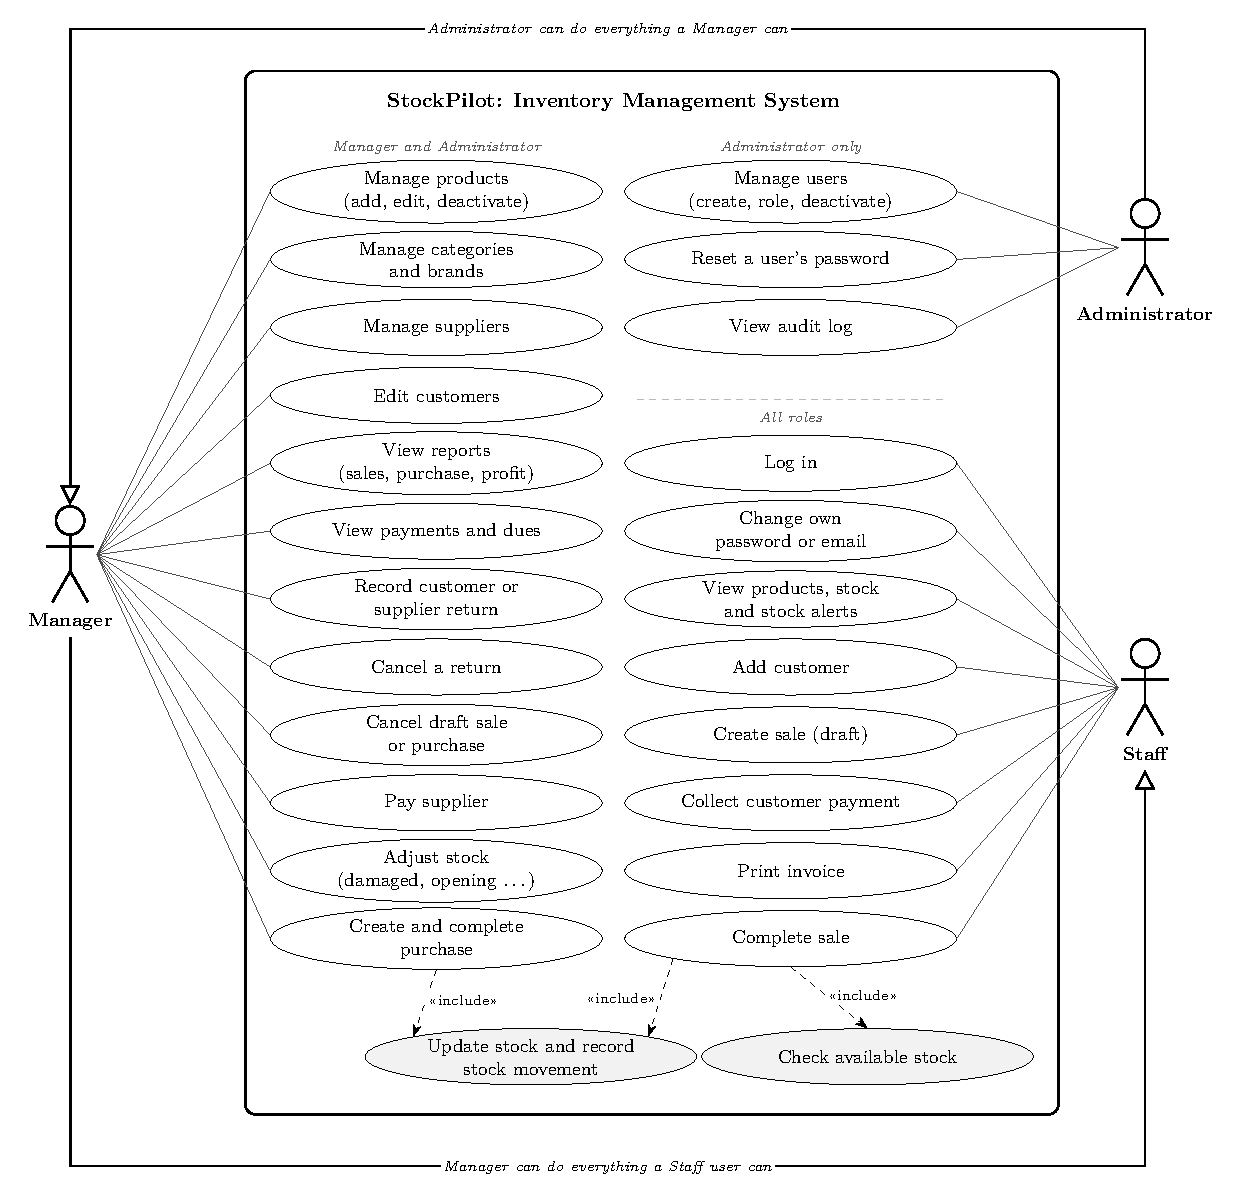
\includegraphics[width=\textwidth]{figures/use-case.pdf}
  \caption{Use case diagram}
\end{figure}

\subsection{Main scenarios}
Six scenarios were written to describe the main business flows from the user's point of view:
\begin{enumerate}
  \item \textbf{Walk-in sale.} A customer without an account buys a product and pays the full amount at once.
  \item \textbf{Credit sale with partial payment.} A known customer buys on credit, pays a part now and the rest later.
  \item \textbf{Purchase and supplier payment.} Products are bought from a supplier, the stock is added, and the supplier is paid in parts.
  \item \textbf{Damaged product and low stock alert.} A broken unit is removed from the stock with a reason, and the product appears in the low stock list.
  \item \textbf{Customer return.} A customer brings a product back; a return saved by mistake can be cancelled.
  \item \textbf{New user.} The Administrator creates a Staff user with a temporary password.
\end{enumerate}

\subsection{Activity diagrams}
A sale and a purchase are both saved first as a \textbf{draft}. A draft does not change the stock. Only when the draft is \textbf{completed}, the stock changes. This makes it possible to prepare a bill, check it, and correct it before it has any effect.
\begin{figure}[H]
  \centering
  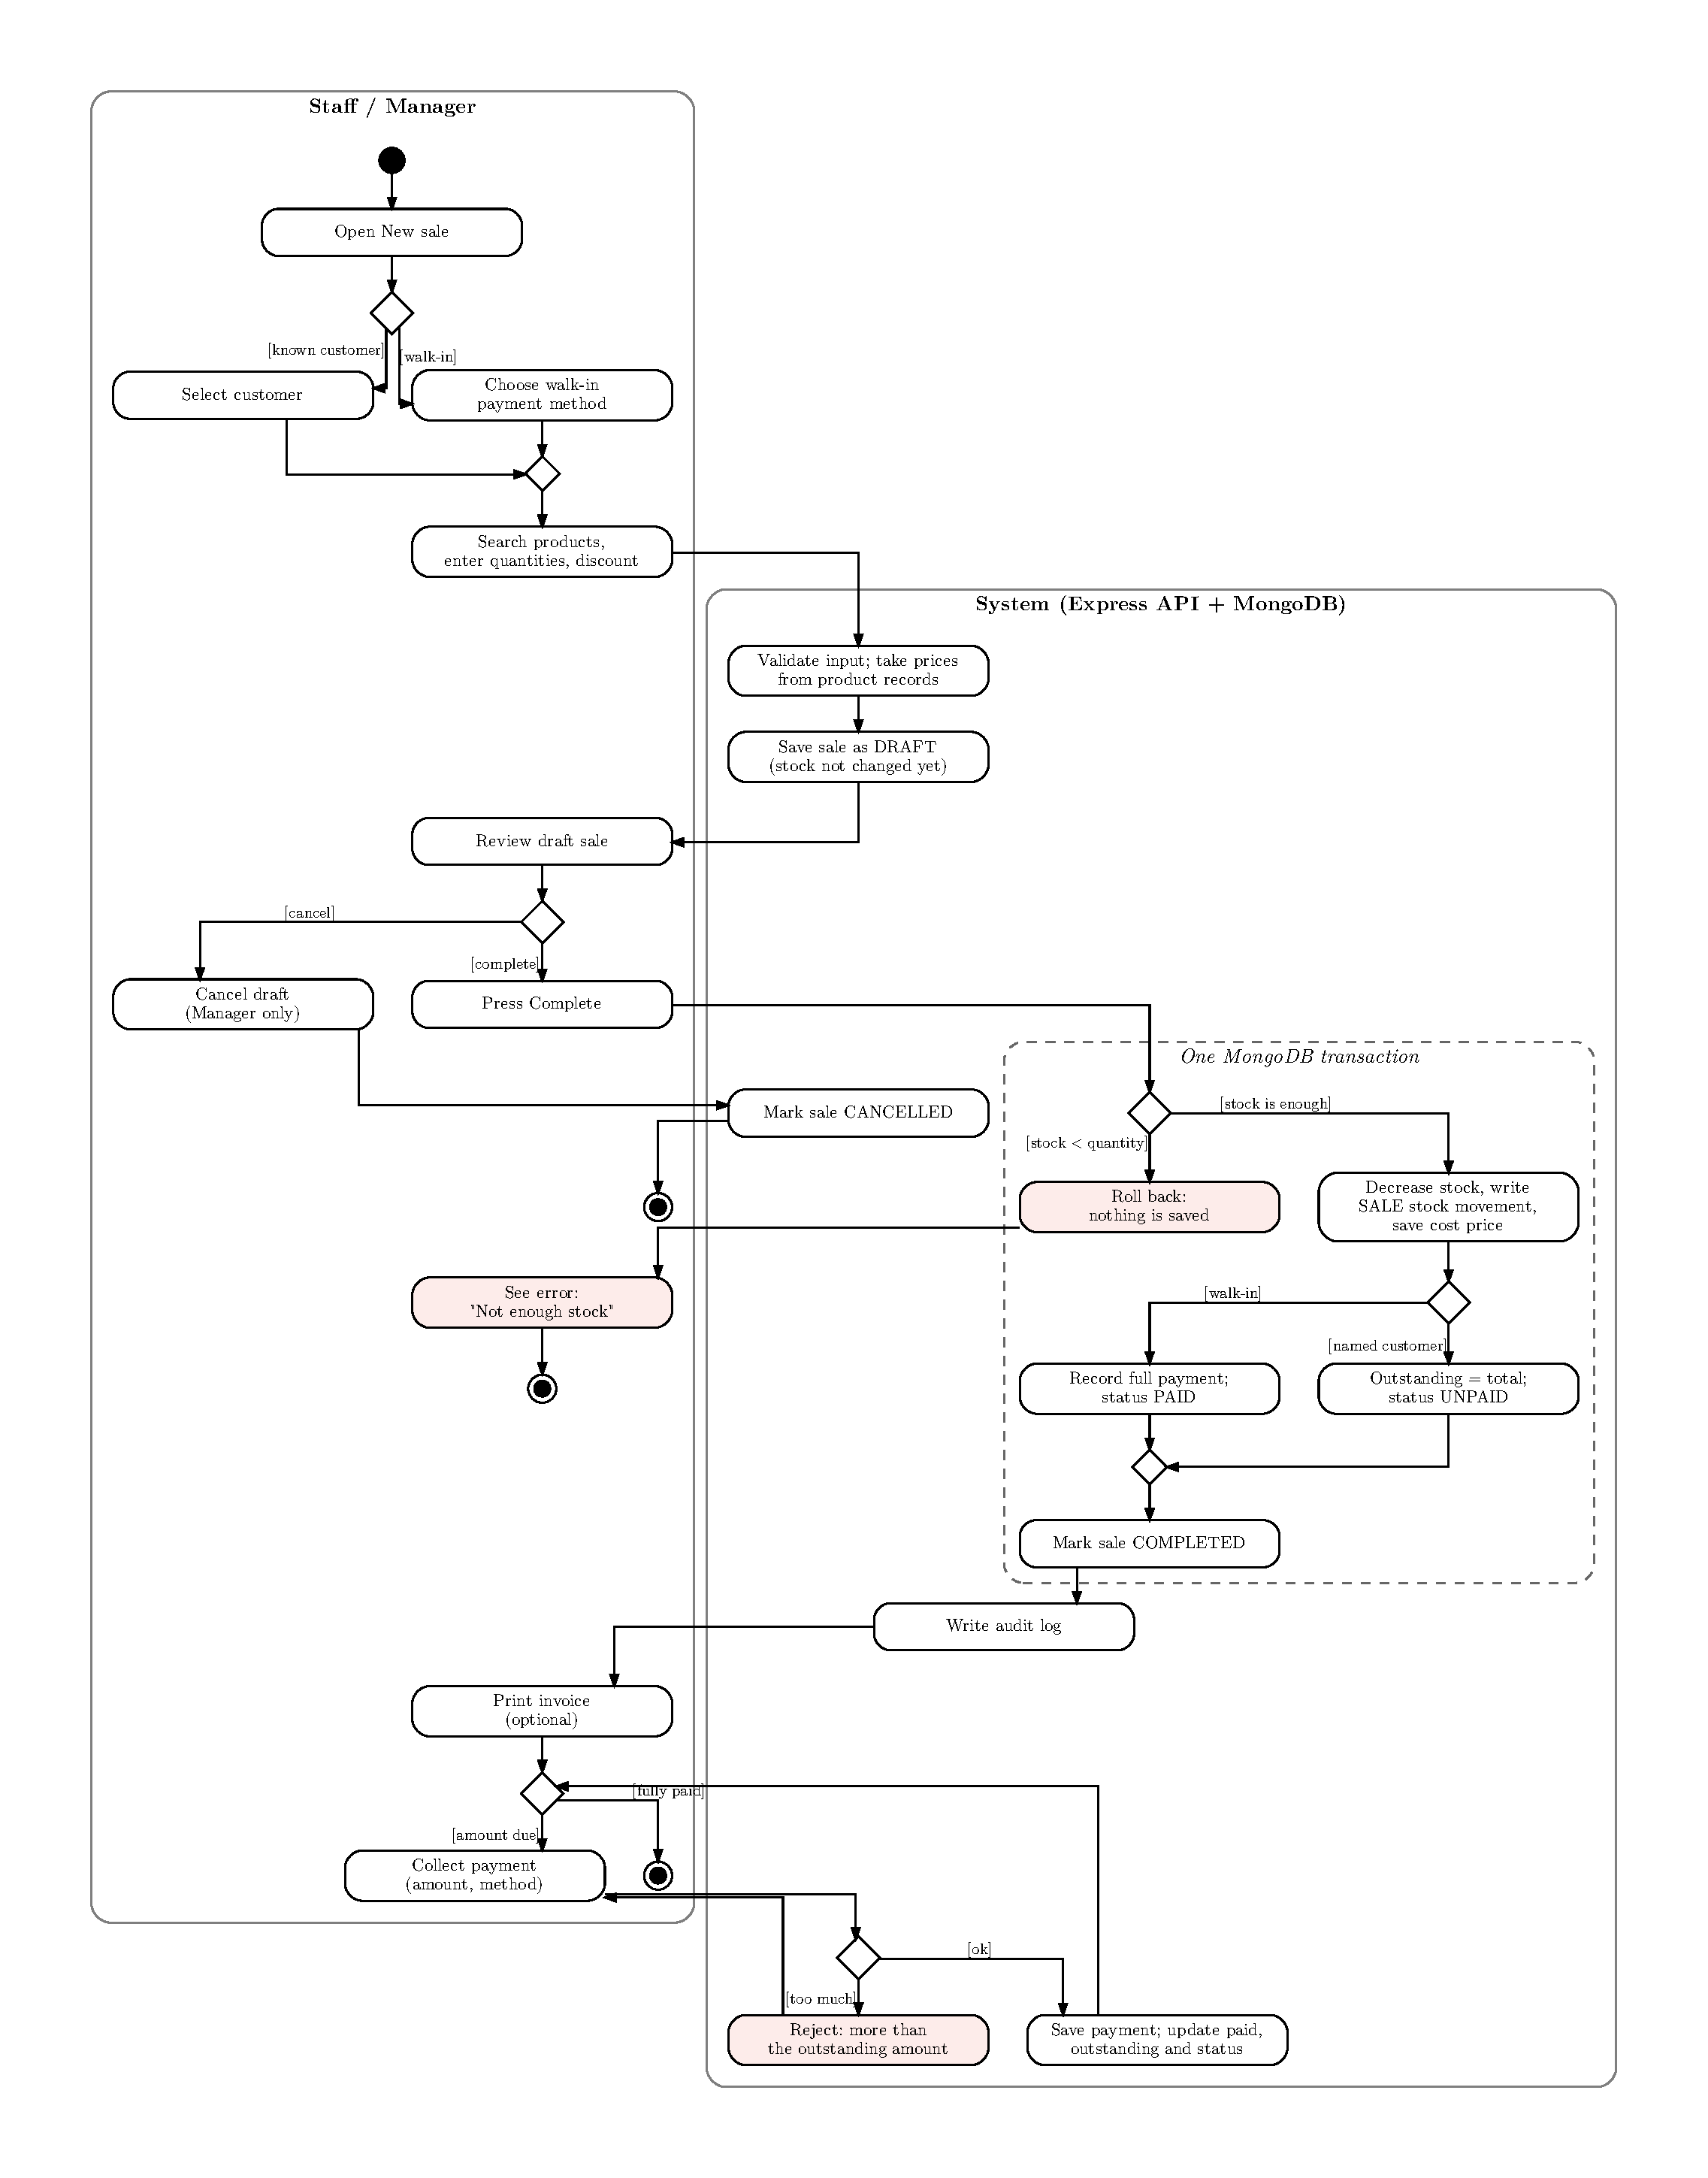
\includegraphics[width=\textwidth,height=0.74\textheight,keepaspectratio]{figures/activity-sale.pdf}
  \caption{Activity diagram: sales process}
\end{figure}
\begin{figure}[H]
  \centering
  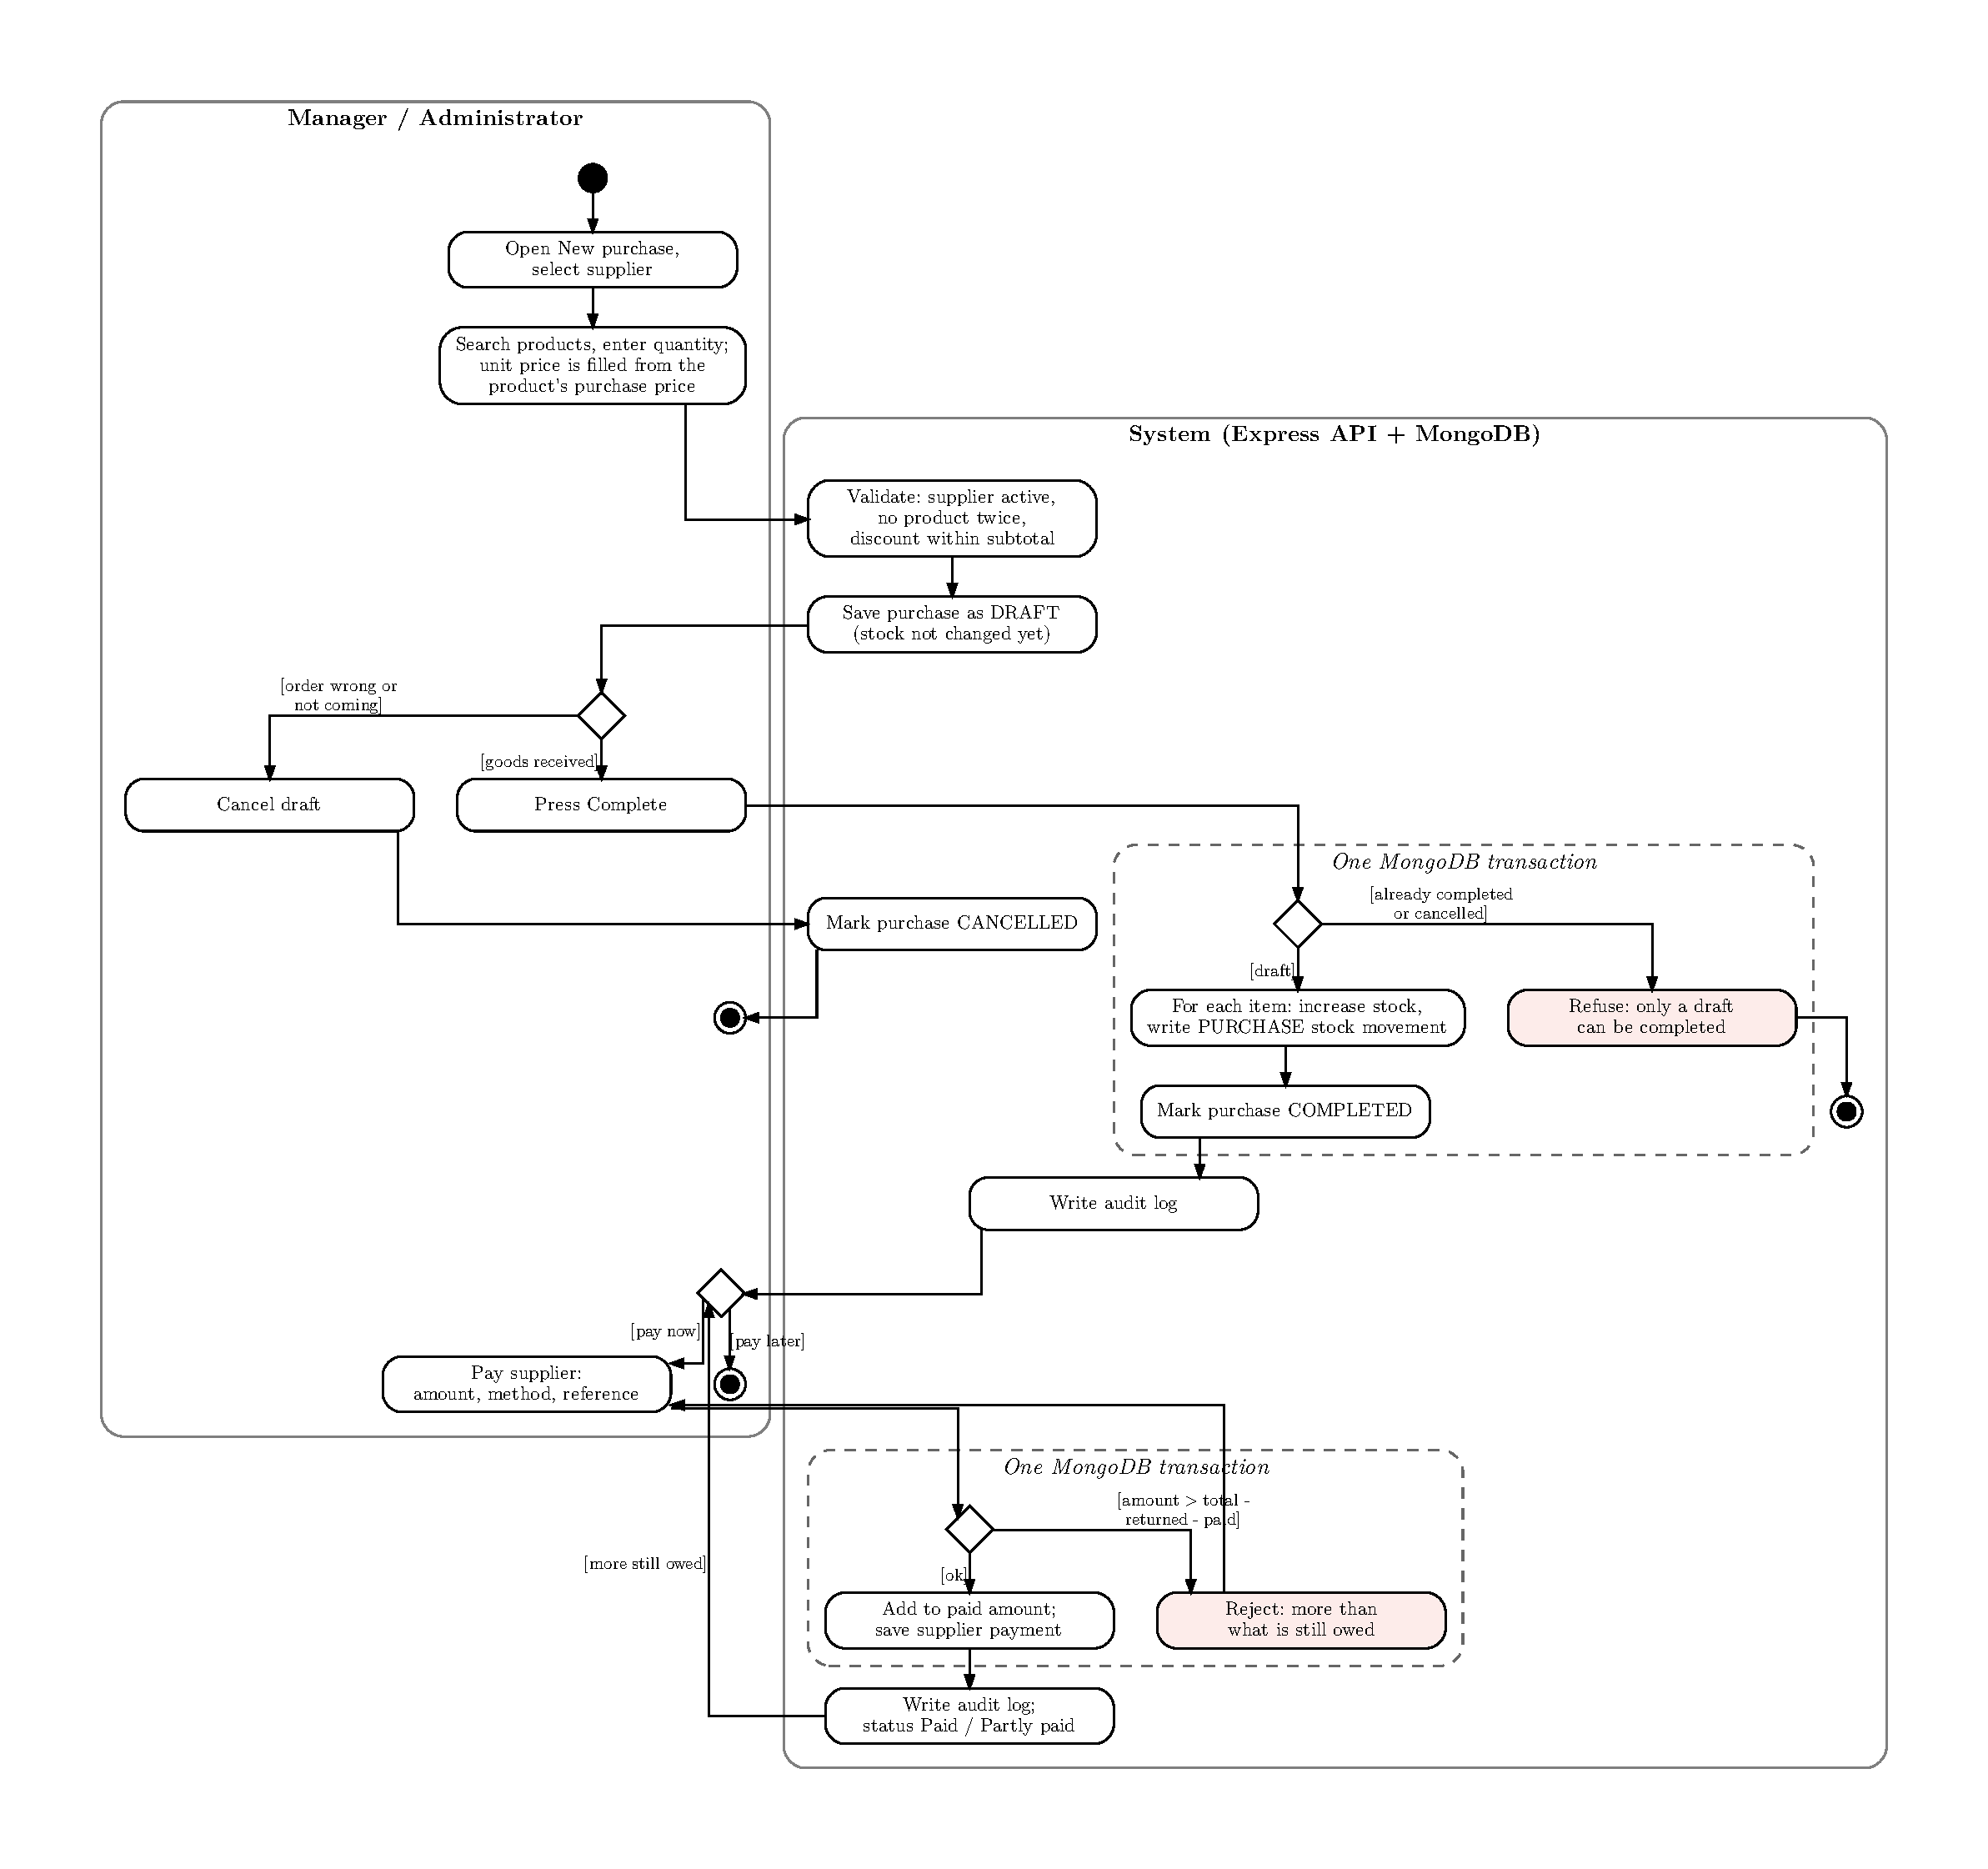
\includegraphics[width=\textwidth,height=0.8\textheight,keepaspectratio]{figures/activity-purchase.pdf}
  \caption{Activity diagram: purchase process}
\end{figure}

\subsection{Class diagram}
\begin{figure}[H]
  \centering
  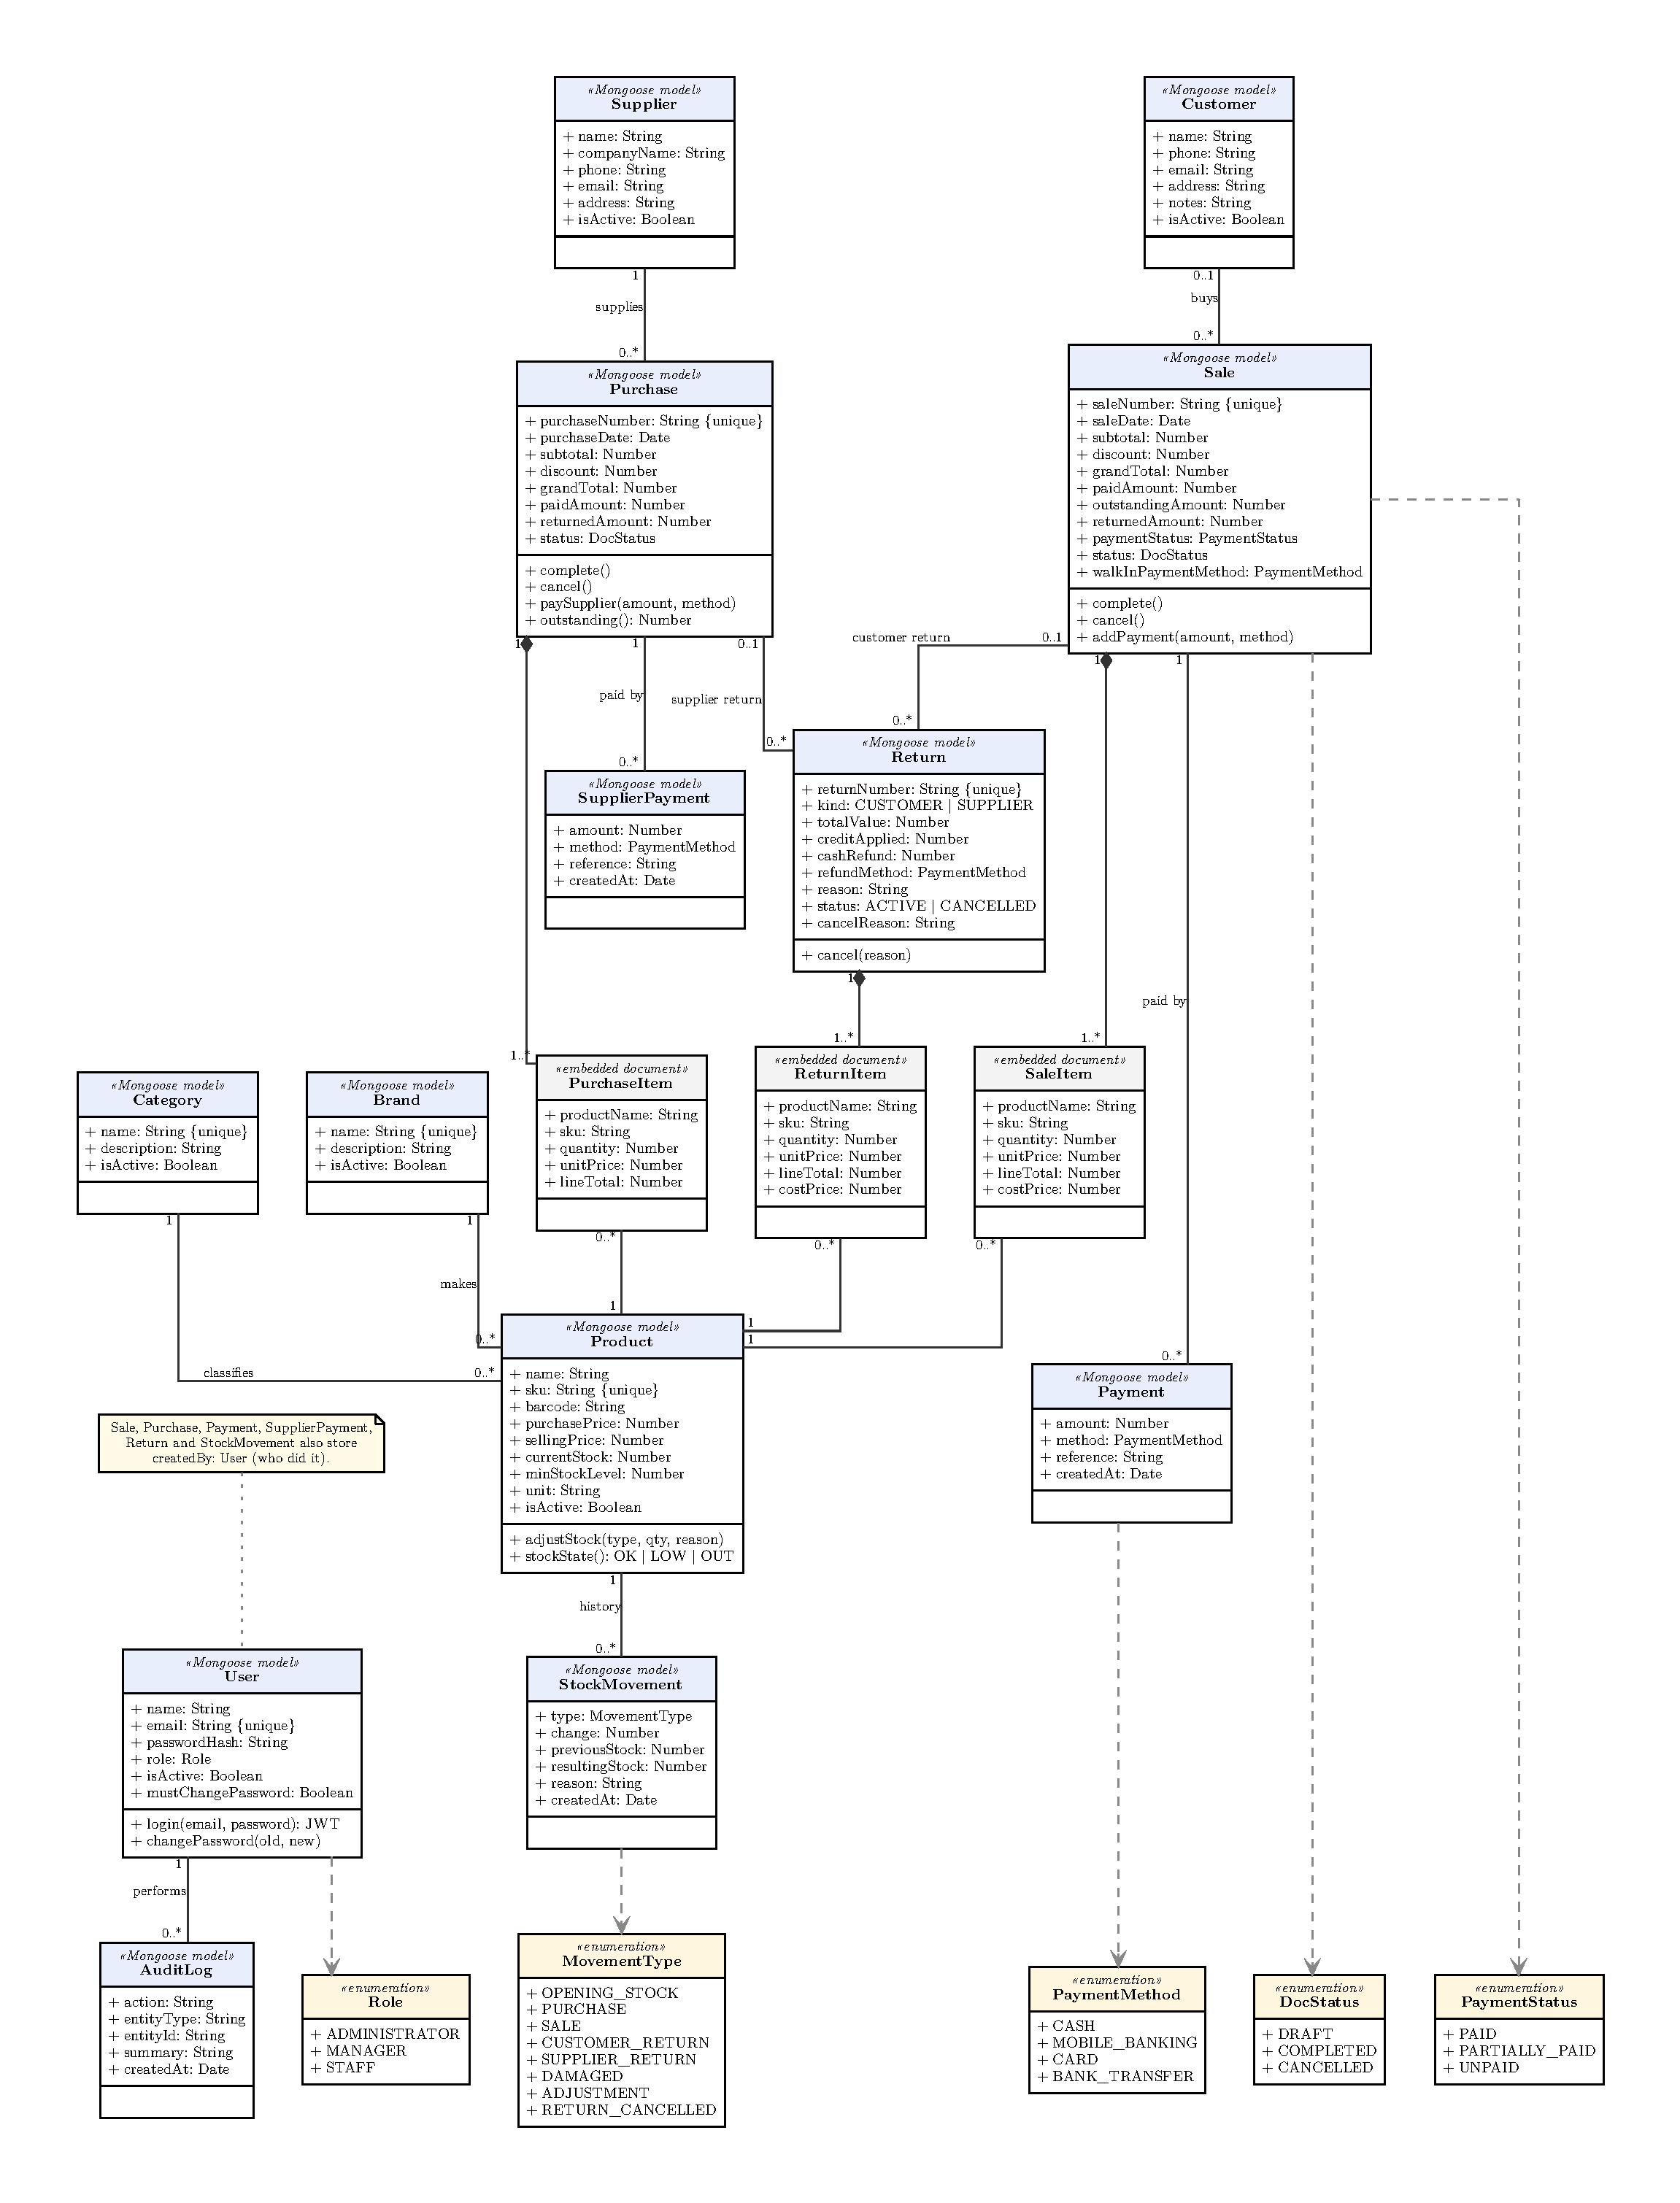
\includegraphics[width=\textwidth,height=0.82\textheight,keepaspectratio]{figures/class-diagram.pdf}
  \caption{Class diagram}
\end{figure}

\subsection{Database diagram}
\begin{figure}[H]
  \centering
  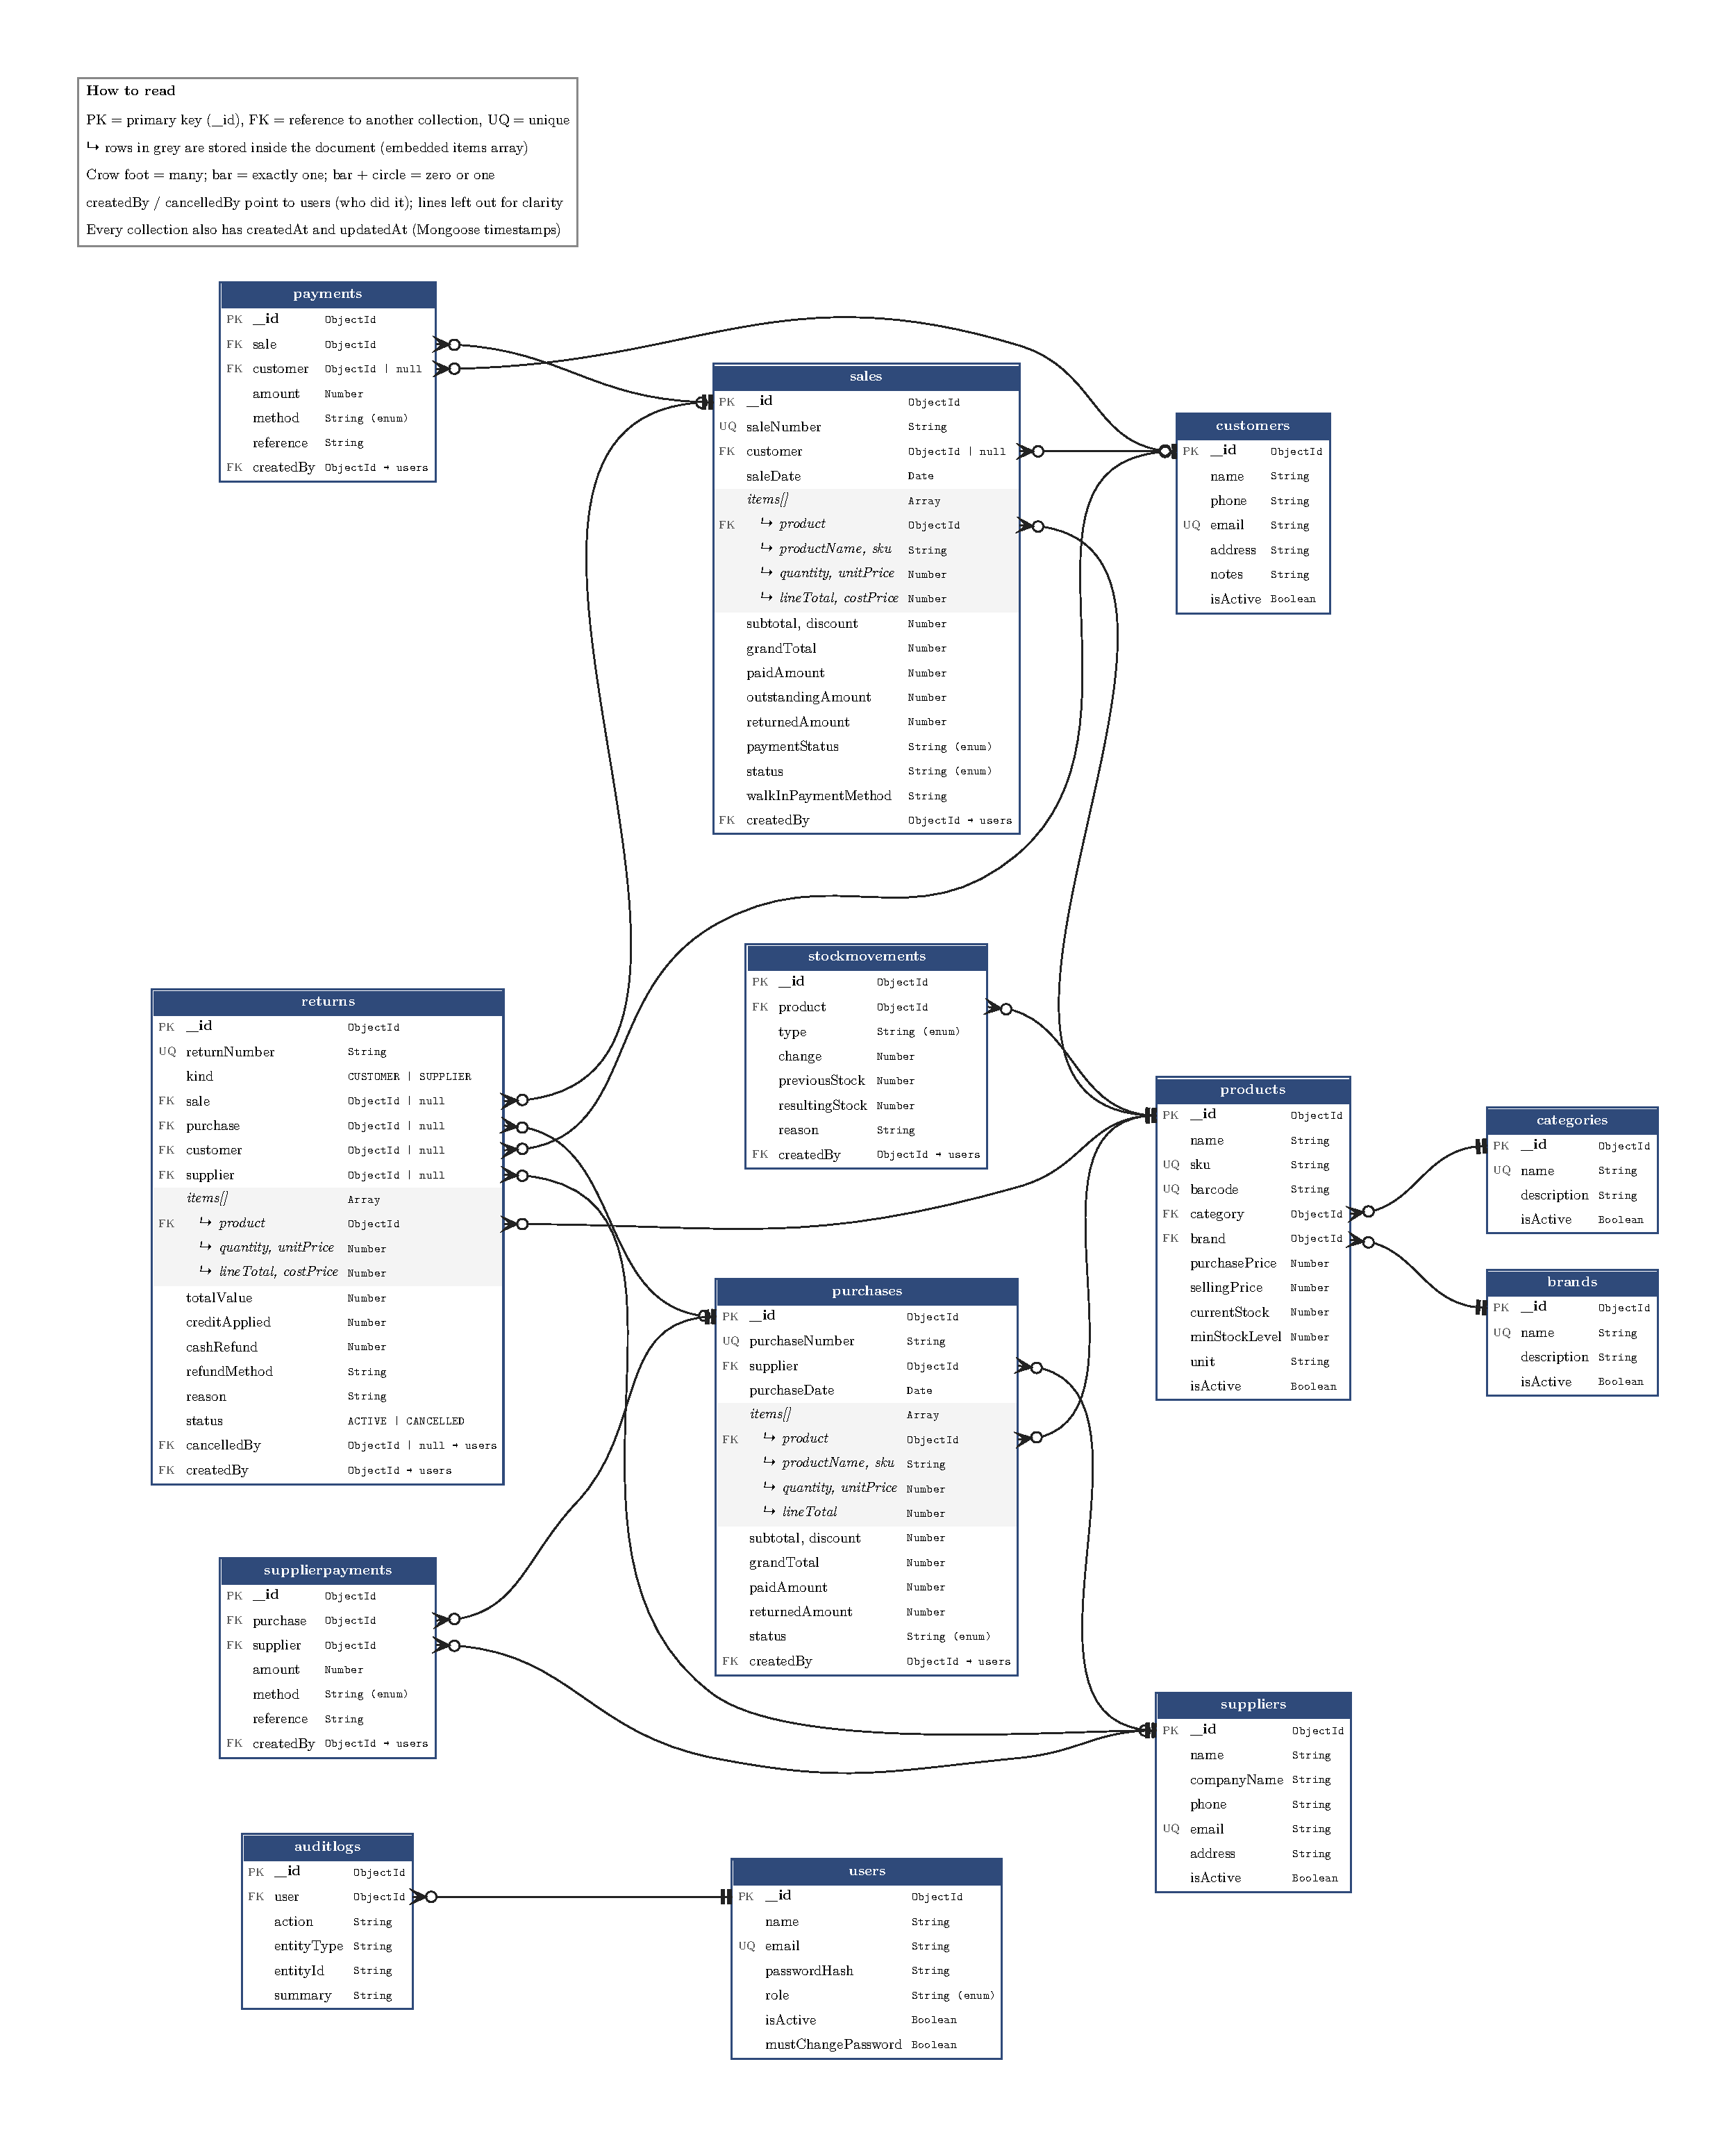
\includegraphics[width=\textwidth,height=0.82\textheight,keepaspectratio]{figures/er-diagram.pdf}
  \caption{Database (ER) diagram of the MongoDB collections}
\end{figure}

\subsection{Design changes from the proposal}
The design was refined while the system was built, as the proposal allowed.
\begin{table}[H]
\centering
\begin{tabularx}{\textwidth}{@{}P{2.7cm}P{4.2cm}Y@{}}
\toprule
\textbf{Topic} & \textbf{Proposal} & \textbf{Final design and reason} \\
\midrule
Roles & Separate \code{roles} collection & A \code{role} field on \code{users} with three fixed values. The roles never change at run time. \\
Line items & Separate item collections & Embedded arrays inside \code{purchases}, \code{sales} and \code{returns}. A bill and its lines are always read and saved together. \\
Invoices & \code{invoices} collection & The printable invoice is generated from the sale, so no copy of the data is stored. \\
Payments & One \code{payments} collection & \code{payments} (from customers) and \code{supplierpayments} (to suppliers), because they have different rules. \\
Batch and expiry & \code{batches} collection & Not in this version. Planned as future work. \\
Returns by Staff & Staff can handle returns & Only Manager and Administrator, because a return changes stock and money. \\
\bottomrule
\end{tabularx}
\caption{Proposal compared with the final design}
\end{table}

% ------------------------------- 3 -------------------------------
\section{Database Implementation}
\subsection{Platform}
The database is MongoDB, hosted on \textbf{MongoDB Atlas}. The cluster is a replica set of three nodes in the AWS Mumbai region, so the data is stored in three copies. The database name is \code{inventory\_management\_system}.

\subsection{Collections}
\begin{table}[H]
\centering
\begin{tabularx}{\textwidth}{@{}P{5.4cm}Y@{}}
\toprule
\textbf{Collection} & \textbf{What it stores} \\
\midrule
\code{users} & User accounts with a role \\
\code{categories}, \code{brands} & Groups of products \\
\code{products} & Products with SKU, prices, current stock and minimum stock level \\
\code{customers}, \code{suppliers} & The people the shop sells to and buys from \\
\code{sales}, \code{payments} & Sales with their lines, and money received from customers \\
\code{purchases}, \code{supplierpayments} & Purchases with their lines, and money paid to suppliers \\
\code{returns} & Products returned by customers or sent back to suppliers \\
\code{stockmovements} & History of every stock change \\
\code{auditlogs} & Who did what and when \\
\bottomrule
\end{tabularx}
\caption{The 13 collections of the database}
\end{table}

\subsection{Schema and rules}
MongoDB creates a collection when the first document is inserted. The structure and the rules of each collection are written as a Mongoose schema in the backend. The schema gives the same protection as constraints in a relational database: required fields, unique values (for example the SKU of a product), minimum values (no negative price or stock) and references to other collections.

\subsection{Queries}
In Step 2, 35 queries were written and executed in a separate practice database: 3 create, 12 read, 6 update, 3 delete, 9 aggregation and 2 index queries. Three techniques from these queries are central to the project.

\textbf{Stock can never go below zero.} The stock is reduced with one conditional update. The filter contains the condition, so the check and the change happen in one step, even when two users sell at the same moment.
\begin{lstlisting}[style=query]
db.products.updateOne(
  { sku: "SAM-S24-001", currentStock: { $gte: 2 } },   // only if 2 are in stock
  { $inc: { currentStock: -2 } }
)
\end{lstlisting}

\textbf{Reports with aggregation.} Totals are calculated inside the database with an aggregation pipeline.
\begin{lstlisting}[style=query]
db.sales.aggregate([
  { $match: { status: "COMPLETED" } },
  { $group: { _id: null,
              count: { $sum: 1 },
              totalSales: { $sum: "$grandTotal" },
              totalPaid: { $sum: "$paidAmount" },
              totalOutstanding: { $sum: "$outstandingAmount" } } }
])
\end{lstlisting}

\textbf{Unique index.} A unique index on \code{sku} stops two products from having the same SKU, and it lets MongoDB find one product among 10,000 by reading a single document.

% ------------------------------- 4 -------------------------------
\section{Backend Development}
\subsection{Technology and structure}
The backend is written in JavaScript with \textbf{Node.js} and \textbf{Express}. Mongoose connects it to MongoDB. The code is split by responsibility:
\begin{lstlisting}[style=query]
server/src/
  server.js      starts Express, adds security and the routes
  routes/        URL + who is allowed            (15 files)
  middleware/    protect (token check), authorize (role check)
  controllers/   validate the input, apply the rules, answer
  models/        Mongoose schemas                (13 files)
\end{lstlisting}

\subsection{How a request is handled}
\begin{enumerate}
  \item \textbf{Route.} Express finds the route that matches the method and the URL.
  \item \textbf{protect.} The token is checked. Without a valid token the answer is 401.
  \item \textbf{authorize.} The role of the user is checked. If the role is not allowed the answer is 403.
  \item \textbf{Controller.} The input is validated (400 for wrong input) and the business rules are applied (409 when a rule is broken, for example not enough stock).
  \item \textbf{Model.} The data is read or changed in MongoDB.
  \item \textbf{Response.} A JSON answer is sent, and the action is written to the audit log.
\end{enumerate}

\subsection{Authentication and security}
\begin{itemize}
  \item \textbf{Passwords} are stored as bcrypt hashes, never as plain text.
  \item \textbf{Login} returns a JWT token that is valid for one day. Every later request sends this token.
  \item The server checks on \textbf{every request} that the user still exists and is active, so a deactivated user is blocked at once.
  \item \textbf{Login attempts} are limited to 10 in 15 minutes.
  \item \textbf{CORS} allows only the address of the frontend, and \code{helmet} adds security headers.
\end{itemize}

\subsection{API overview}
All paths start with \code{/api/v1}. The complete list of the 55 routes is in the Step 3 document.
\begin{table}[H]
\centering
\begin{tabularx}{\textwidth}{@{}P{4.4cm}cY@{}}
\toprule
\textbf{Module} & \textbf{Routes} & \textbf{Main functions} \\
\midrule
Health and authentication & 3 & Server check, login, current user \\
Users and accounts & 7 & Create users, roles, passwords, email \\
Categories and brands & 6 & List, create, update \\
Products & 4 & List with search and pages, create, update \\
Customers and suppliers & 6 & List with search, create, update \\
Inventory & 3 & Stock adjustment, stock history, alerts \\
Purchases & 7 & Draft, complete, cancel, supplier payments \\
Sales and payments & 8 & Draft, complete, cancel, customer payments \\
Returns & 6 & Customer return, supplier return, cancel a return \\
Reports and audit log & 5 & Sales, purchases, stock value, profit, audit log \\
\midrule
Total & 55 & \\
\bottomrule
\end{tabularx}
\caption{API routes by module}
\end{table}

\subsection{Transactions}
Some actions change several collections. Completing a sale reduces the stock of each product, writes the stock history and updates the sale. These changes run inside one MongoDB transaction. If one step fails, for example because one product has too little stock, all changes are cancelled. The database is never left in a half-finished state.

% ------------------------------- 5 -------------------------------
\section{Frontend Development}
\subsection{Technology and structure}
The frontend is built with \textbf{React 19}, \textbf{Next.js 16}, \textbf{TypeScript} and \textbf{Tailwind CSS}. It is a single-page application: the browser loads it once, and after that only data is exchanged with the backend.
\begin{itemize}
  \item \code{auth-gate.tsx} shows the login form when there is no valid token.
  \item \code{app/page.tsx} shows the sidebar, the top bar and the open page.
  \item One component for each page loads its own data and shows tables, filters and buttons.
  \item Modal components hold the forms and the detail windows.
\end{itemize}

\subsection{Pages}
\begin{table}[H]
\centering
\begin{tabularx}{\textwidth}{@{}P{2.4cm}Y@{}}
\toprule
\textbf{Menu group} & \textbf{Pages} \\
\midrule
Overview & Dashboard \\
Catalog & Products, Categories, Brands \\
Operations & Inventory, Purchases, Sales \\
People & Customers, Suppliers \\
Finance & Returns, Payments and Dues, Reports \\
System & User Management, Audit Log \\
\bottomrule
\end{tabularx}
\caption{The 14 pages of the frontend}
\end{table}

\subsection{Connection with the backend}
All requests go through one function, \code{apiRequest} in \code{lib/api.ts}. It adds the backend address and the token, turns the data into JSON, and turns every failed answer into an error with the message of the server. The frontend uses 52 of the 55 routes.

The address of the backend comes from the environment variable \code{NEXT\_PUBLIC\_API\_BASE\_URL}, so the same code works on a local computer and on the internet.

The user interface follows the role of the user: buttons that the role may not use are hidden. This is only for a clear interface. The real protection is in the backend, which checks the role on every request.

\subsection{Screenshots}
\shot{dashboard.png}{Dashboard with live figures from the backend}
\shot{products.png}{Products page with search, filters and pages (more than 10,000 products)}
\shot{purchases.png}{Purchases page: the buttons depend on the status of the purchase}
\shot[0.7]{new-sale.png}{New sale form with the product search box}
\shot{payments.png}{Payments and Dues page}
\shot{staff-view.png}{A Staff user opens Purchases: the page explains that there is no permission}
\shot{network.png}{Browser DevTools: the page (port 3000) requests its data from the backend API (port 5000)}

% ------------------------------- 6 -------------------------------
\section{System Integration and Testing}
\subsection{Integration}
The three parts are joined by three settings:
\begin{table}[H]
\centering
\begin{tabularx}{\textwidth}{@{}P{3.2cm}P{5.2cm}Y@{}}
\toprule
\textbf{Connection} & \textbf{Setting} & \textbf{Where} \\
\midrule
Frontend to backend & \code{NEXT\_PUBLIC\_API\_BASE\_URL} & Frontend \\
Backend allows frontend & \code{CLIENT\_URL} (CORS) & Backend \\
Backend to database & \code{MONGO\_URI} & Backend \\
\bottomrule
\end{tabularx}
\caption{Settings that connect the three parts}
\end{table}
The integration was done from the bottom up: first the backend with the database, then the frontend with the backend.

All tests that create or change data run in a separate test environment with its own database (\code{stockpilot\_api\_test}). The real data is never changed by a test.

\subsection{Test levels and results}
\begin{table}[H]
\centering
\begin{tabularx}{\textwidth}{@{}P{2.6cm}P{2.6cm}YP{2.6cm}@{}}
\toprule
\textbf{Level} & \textbf{Tool} & \textbf{What is tested} & \textbf{Result} \\
\midrule
Unit tests & Vitest & Token check, role check, login limit, input validation & 19 of 19 passed \\
Integration tests & Vitest + MongoDB & Backend with a real database; also two requests at the same moment & 8 of 8 passed \\
API tests & Postman & All 55 routes: 92 requests, 217 checks & 217 of 217 passed \\
System tests & By hand, in the browser & The whole system as a user works: 27 cases & 21 passed, 6 not run \\
Deployment tests & By hand, live website & The three parts on three servers: 3 cases & Not run \\
\bottomrule
\end{tabularx}
\caption{Test levels and results}
\end{table}

\shot{postman-result.png}{Result of the Postman collection run: 217 checks passed, 0 failed}

\subsection{System test: one product through its whole life}
In the system test one product was followed from purchase to return. After every step the stock and the amounts of money on the website were compared with the expected values.
\begin{table}[H]
\centering
\begin{tabular}{@{}lrr@{}}
\toprule
\textbf{Action} & \textbf{Stock} & \textbf{Customer due (Tk)} \\
\midrule
Product created & 0 & -- \\
Purchase of 10 completed & 10 & -- \\
Sale of 2 on credit completed & 8 & 42,000 \\
Customer pays 20,000 & 8 & 22,000 \\
Sale of 50 refused (not enough stock) & 8 & 22,000 \\
Walk-in sale of 1, paid at once & 7 & 22,000 \\
1 unit damaged & 6 & 22,000 \\
Customer returns 1 & 7 & 1,000 \\
Return cancelled & 6 & 22,000 \\
\bottomrule
\end{tabular}
\caption{Stock and due amount after each step of the system test}
\end{table}
At the end the report pages showed sales of Tk 63,000, purchases of Tk 180,000, a gross profit of Tk 9,000 and a stock value of Tk 108,000. All values were the same as calculated by hand.
\shot{reports-s22.png}{Reports page at the end of the system test}

The six system cases and the three deployment cases that are marked \emph{not run} check roles in the browser, the session, a server failure, the audit log and the live website. The rules behind them (roles and error handling) are already covered by the API tests.

% ------------------------------- 7 -------------------------------
\section{Deployment}
\begin{table}[H]
\centering
\begin{tabularx}{\textwidth}{@{}P{2.4cm}P{3cm}Y@{}}
\toprule
\textbf{Part} & \textbf{Service} & \textbf{Location} \\
\midrule
Frontend & Vercel & Global network \\
Backend & Render & Oregon, USA \\
Database & MongoDB Atlas & Mumbai, India (AWS) \\
\bottomrule
\end{tabularx}
\caption{The three parts run on three different servers in different places}
\end{table}
The browser loads the frontend from Vercel, the frontend calls the backend on Render, and the backend reads and writes the database on Atlas.
\begin{itemize}
  \item Live website: \url{https://inventory-management-system-rouge-nu.vercel.app}
  \item Source code: \url{https://github.com/mdraihan2010/inventory-management-system}
\end{itemize}

% ------------------------------- 8 -------------------------------
\section{Limitations and Future Work}
\subsection{Limitations}
\begin{itemize}
  \item A return that included a cash refund cannot be cancelled. A new sale is recorded instead.
  \item When a supplier has been paid in full and products are returned afterwards, the money that the supplier owes back is not tracked.
  \item The free backend server sleeps when it is not used, so the first request after a pause is slow.
  \item The system tests are done by hand.
  \item Batch and expiry tracking, which the proposal mentioned, is not part of this version.
\end{itemize}

\subsection{Future work}
\begin{itemize}
  \item Batch and expiry dates for products.
  \item Barcode scanning in the sale form.
  \item Automatic browser tests for the system test cases.
  \item Support for several branches of a shop.
  \item Export of reports as PDF.
\end{itemize}

% ------------------------------- 9 -------------------------------
\section{Conclusion}
The objectives of the project were reached. The Inventory Management System keeps products, stock, purchases, sales, payments and returns in one place. The stock is updated automatically and can never go below zero, the dues of customers and suppliers are always known, and each user can do only what the role allows.

The project also showed how a modern web application is built in layers: a database with clear rules, a backend that protects these rules behind an API, and a frontend that uses only this API. Because each layer was tested alone before the layers were joined, problems were found early and were easy to locate.

% ------------------------------- References -------------------------------
\section*{References}
\addcontentsline{toc}{section}{References}
\begin{enumerate}[label={[\arabic*]}]
  \item MongoDB Documentation. \url{https://www.mongodb.com/docs/}
  \item Mongoose Documentation. \url{https://mongoosejs.com/docs/}
  \item Express Documentation. \url{https://expressjs.com/}
  \item Node.js Documentation. \url{https://nodejs.org/docs/}
  \item React Documentation. \url{https://react.dev/}
  \item Next.js Documentation. \url{https://nextjs.org/docs}
  \item Postman Learning Center. \url{https://learning.postman.com/}
  \item JSON Web Token Introduction. \url{https://jwt.io/introduction}
\end{enumerate}

% ------------------------------- Appendix -------------------------------
\appendix
\section{Detailed Documents}\label{app:documents}
Each step has a detailed document in the folder \code{docs} of the repository.
\begin{table}[H]
\centering
\begin{tabularx}{\textwidth}{@{}clY@{}}
\toprule
\textbf{Step} & \textbf{File} & \textbf{Contents} \\
\midrule
1 & \code{docs/design/system-design.pdf} & Scenarios and all diagrams \\
2 & \code{docs/database/database-queries.pdf} & 35 queries with expected results \\
3 & \code{docs/api/api-testing.pdf} & 55 routes and 92 Postman test cases \\
4 & \code{docs/frontend/frontend.pdf} & Pages, connection and screenshots \\
5 & \code{docs/testing/system-testing.pdf} & Test plan and 27 system test cases \\
\bottomrule
\end{tabularx}
\caption{Detailed documents of the project}
\end{table}

\end{document}
